\section{Setup and Procedure}
The experimental setup consists of tube (see figure~\ref{fig:setup1}) being
isolated both thermal and in terms of magnetic fields. 
The photography shows the experimental setup, where the squid is operating inside the tube in order
    to screen perturbative magnetic fields and thermal fluctuations. The tube is cooled down
    with liquid nitrogen in order to establish the superconduction. In the lower part of the
    tube is additional space not being cooled down by the nitrogen for the objects to be inserted.
    The magnetic fields of these objects will then be measured by the squid.
First we use a conductor loop, which will be rotated in a certain frequency with
an external drive. The Squid is connected with an oscilloscope such that 
we can track the magnetic field continuously.
\begin{figure}[htpb]
    \centering
    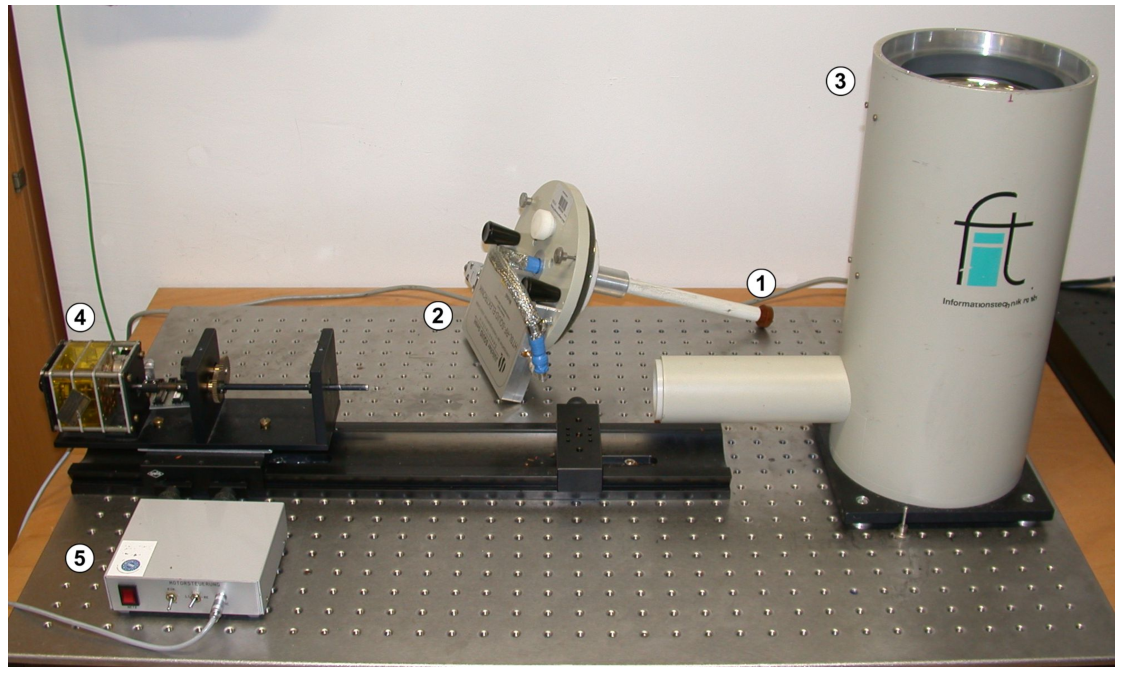
\includegraphics[width=0.8\linewidth]{figures/setup_fig}
    \caption{Figure taken from \cite{ver}. (1) SQUID ring (2) SQUID control (3) cryostat (4) gear and 
    rail for movement of sample (5) control of gear}
    \label{fig:setup1}
\end{figure}
\paragraph{The procedure} of conducting the experiment will be
the following:
\begin{enumerate}
\item Filling the tube with liquid nitrogen in order to establish the superconduction in the
operating squid, which will take about 15 minutes.
\item Calibration of the squid by means of the visible amplitude in the oscilloscope \textit{Hameg 1508-2}.
Maximizing the quality of the signal with the amplitude VCA and the frequency VCO of the oscillating circuit, as
well as setting the offset to zero by using the option OFF.
\item Measuring the magnetic field of the oscillating RLC unit with different resistances.
\item Measuring the magnetic fields of various other objects.
\end{enumerate}


